\documentclass[a4paper]{article}
\usepackage[a4paper,margin=0mm]{geometry}
\usepackage{fontspec}
\usepackage{unicode-math}
\usepackage{tikz}
\usetikzlibrary{fit,calc,positioning,arrows.meta}
\usepackage[table]{xcolor}
\usepackage[absolute]{textpos}
\usepackage{array}

\setmainfont{Libertinus Serif}
\setsansfont{Libertinus Sans}
\setmathfont{Libertinus Math}

\definecolor{accent}{HTML}{602785}
\definecolor{badge}{HTML}{B8A0C8}
\definecolor{ink}{HTML}{2A2E30}

\setlength{\TPHorizModule}{1mm}
\setlength{\TPVertModule}{1mm}
\setlength{\parindent}{0pt}
\pagestyle{empty}

\newcommand{\topicheader}[2]{%
\begin{textblock*}{194mm}(16mm,10mm)
\begin{tikzpicture}
\node[fill=accent,text=white,font=\sffamily\bfseries\fontsize{13}{13}\selectfont,
      minimum width=9mm,minimum height=9mm,inner sep=0pt] at (4.5mm,-4.5mm) {#1};
\node[font=\sffamily\bfseries\fontsize{15}{16}\selectfont,text=ink,anchor=west] at (12mm,-4.5mm) {#2};
\end{tikzpicture}
\end{textblock*}
\begin{textblock*}{194mm}(16mm,22.5mm)

\begin{tikzpicture}
\fill[accent] (0,0) rectangle (194mm,0.5mm);
\end{tikzpicture}
\end{textblock*}
}

\newcommand{\pagekicker}[1]{%
\begin{textblock*}{100mm}(16mm,25.5mm)
\begin{tikzpicture}
\node[fill=ink,text=white,font=\sffamily\bfseries\fontsize{8}{8}\selectfont,
      inner sep=2.2pt,rounded corners=1pt] {\MakeUppercase{#1}};
\end{tikzpicture}
\end{textblock*}
}

\newcommand{\videobanner}[1]{%
\begin{textblock*}{178mm}(16mm,25.5mm)
\begin{tikzpicture}
\fill[accent] (0,0) rectangle (178mm,-10mm);
\draw[white,line width=0.6pt] (3mm,-1.7mm) rectangle (11.5mm,-8.3mm);
\node[white,font=\sffamily\fontsize{4}{4.4}\selectfont,align=center] at (7.25mm,-5mm) {QR\\CODE};
\node[white,font=\sffamily\bfseries\fontsize{9.5}{11}\selectfont,anchor=west] at (16mm,-5.6mm) {WATCH THE VIDEO BEFORE YOU SOLVE};
\node[white,font=\sffamily\fontsize{7.5}{8}\selectfont,anchor=east] at (174mm,-5.6mm) {YouTube ~\textbullet~ #1};
\end{tikzpicture}
\end{textblock*}
}

\newcommand{\pagefooter}[1]{%
\begin{textblock*}{194mm}(8mm,286.41mm)
  
\begin{tikzpicture}
    \fill[accent] (0,0) rectangle (194mm,0.6mm);
  \end{tikzpicture}
\end{textblock*}
\begin{textblock*}{63.59mm}(8mm,288.27mm)
  {\sffamily\bfseries\color{accent}\fontsize{13}{16}\selectfont SAT 1200+}
\end{textblock*}
\begin{textblock*}{10mm}(188mm,288.27mm)
  \centering{\sffamily\color{accent}\fontsize{14}{16}\selectfont #1}
\end{textblock*}
}

\newcommand{\cardbg}[4]{%
\begin{textblock*}{#3mm}(#1mm,#2mm)
\begin{tikzpicture}
\fill[badge!22,rounded corners=3mm] (0,0) rectangle (#3mm,-#4mm);
\end{tikzpicture}
\end{textblock*}%
}

\newcommand{\pill}[3]{%
\begin{textblock*}{160mm}(#1mm,#2mm)
\begin{tikzpicture}
\node[fill=accent,text=white,anchor=north west,font=\sffamily\bfseries\fontsize{10}{10}\selectfont,
      rounded corners=8pt,inner xsep=5mm,inner ysep=1.8mm] at (0,0) {RULE ~\textperiodcentered~ #3};
\end{tikzpicture}
\end{textblock*}%
}

\arrayrulecolor{accent}
\setlength{\arrayrulewidth}{0.7pt}
\renewcommand{\arraystretch}{1.5}

\begin{document}

% ======================================================================
% PAGE 1
% ======================================================================
\topicheader{16}{Data Representations}
\videobanner{Lesson 16}
\pagefooter{84}
\mbox{}%

% ---- CARD 1: Frequency table ----
\cardbg{16}{40}{178}{45}
\pill{26}{43}{Frequency table (chastota jadvali)}

\begin{textblock*}{158mm}(26mm,56mm)
{\fontsize{11}{14}\selectfont\color{ink}
Total = sum of all frequencies. Percent of a category $=\dfrac{\text{count}}{\text{total}}\times100\%$.}
\end{textblock*}

\begin{textblock*}{158mm}(26mm,72mm)
{\fontsize{12}{15}\selectfont
$18$ of $50$ students: $\dfrac{18}{50}\times100\%=36\%$}
\end{textblock*}

% ---- CARD 2: Two-way table ----
\cardbg{16}{93}{178}{115}
\pill{26}{96}{Two-way table -- pick the right denominator}

\begin{textblock*}{110mm}(26mm,109mm)
{\fontsize{10}{13}\selectfont
\begin{tabular}{|p{24mm}|>{\centering\arraybackslash}p{20mm}|>{\centering\arraybackslash}p{20mm}|>{\centering\arraybackslash}p{24mm}|}
\hline
\rowcolor{accent}
{\color{white}} & {\color{white}Basketball} & {\color{white}Volleyball} & {\color{white}Row total} \\ \hline
Girls & 14 & 26 & \textbf{40} \\ \hline
Boys & 33 & 17 & \textbf{50} \\ \hline
\textbf{Col. total} & \textbf{47} & \textbf{43} & \textbf{90} \\ \hline
\end{tabular}}
\end{textblock*}

\begin{textblock*}{158mm}(26mm,146mm)
{\fontsize{10.5}{13}\selectfont\color{ink}
``\% of girls'' $\to$ denominator = girls' row total. ``\% of volleyball
choosers'' $\to$ denominator = volleyball's column total.}
\end{textblock*}

\begin{textblock*}{158mm}(26mm,162mm)
{\fontsize{11}{14}\selectfont
\% of girls who chose volleyball: $\dfrac{26}{40}\times100\%=65\%$}
\end{textblock*}

\begin{textblock*}{158mm}(26mm,176mm)
{\fontsize{11}{14}\selectfont
\% of volleyball choosers who are girls: $\dfrac{26}{43}\times100\%\approx60.5\%$}
\end{textblock*}

\begin{textblock*}{158mm}(26mm,192mm)
{\fontsize{10}{13}\selectfont\color{black!55}\itshape
Same number ($26$), different denominator, different answer -- read the
question's word order carefully.}
\end{textblock*}

\clearpage

% ======================================================================
% PAGE 2
% ======================================================================
\topicheader{16}{Data Representations}
\pagekicker{Rules sheet -- 2/2}
\pagefooter{85}
\mbox{}%

% ---- CARD 3: Scatterplot ----
\cardbg{16}{33}{178}{145}
\pill{26}{36}{Scatterplot -- correlation}

\begin{textblock*}{158mm}(26mm,49mm)
{\fontsize{11}{14}\selectfont
\begin{tabular}{|p{80mm}|>{\centering\arraybackslash}p{70mm}|}
\hline
\rowcolor{accent}
{\color{white}\textbf{Pattern}} & {\color{white}\textbf{Correlation}} \\ \hline
Points trend up, left to right & Positive \\ \hline
Points trend down, left to right & Negative \\ \hline
No clear up/down trend & None \\ \hline
\end{tabular}}
\end{textblock*}

\begin{textblock*}{100mm}(26mm,97mm)
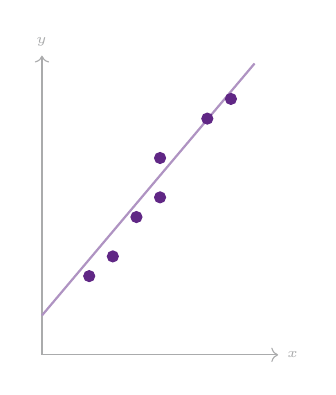
\begin{tikzpicture}
\draw[ink!40,->] (0,0) -- (30mm,0) node[right,font=\tiny]{$x$};
\draw[ink!40,->] (0,0) -- (0,38mm) node[above,font=\tiny]{$y$};
\draw[accent!50,line width=0.8pt] (0,5mm) -- (27mm,37mm);
\filldraw[accent] (6mm,10mm) circle (0.7mm);
\filldraw[accent] (9mm,12.5mm) circle (0.7mm);
\filldraw[accent] (12mm,17.5mm) circle (0.7mm);
\filldraw[accent] (15mm,20mm) circle (0.7mm);
\filldraw[accent] (15mm,25mm) circle (0.7mm);
\filldraw[accent] (21mm,30mm) circle (0.7mm);
\filldraw[accent] (24mm,32.5mm) circle (0.7mm);
\end{tikzpicture}
\end{textblock*}

\begin{textblock*}{70mm}(135mm,110mm)
{\fontsize{10}{13}\selectfont\color{ink}
Points rise left to right $\to$ \textbf{positive correlation}.}
\end{textblock*}

\begin{textblock*}{158mm}(26mm,146mm)
{\fontsize{10.5}{13}\selectfont\color{ink}
SAT asks for the relationship in words (``strong positive,'' ``weak
negative,'' ``no correlation''), not an $r$-value formula.}
\end{textblock*}

\begin{textblock*}{158mm}(26mm,162mm)
{\fontsize{10}{13}\selectfont\color{black!55}\itshape
Correlation is not causation -- a trend between two quantities does not
prove one causes the other.}
\end{textblock*}

\end{document}
